\documentclass{article}
\usepackage[frenchb]{babel}
\usepackage{amsfonts}
\usepackage{amsmath}
\usepackage[T1]{fontenc}
\usepackage[utf8]{inputenc}
\usepackage{amsthm}
\usepackage{graphicx}
\usepackage{subfigure}

\title{Apprentissage Statistique en Génomique}
\author{Dell'Aiera Clément, Prévosteau Clément}
\date{}

\newtheorem{definition}{Def}
\newtheorem{thm}{Théorème}
\newtheorem{ex}{Exercice}
\newtheorem{lem}{Lemme}
\newtheorem{dem}{Preuve}
\newtheorem{prop}{Proposition}
\newtheorem{cor}{Corollaire}

\newcommand{\Z}{\mathbb Z}
\newcommand{\R}{\mathbb R}
\newcommand{\C}{\mathbb C}
\newcommand{\Hil}{\mathcal H}
\newcommand{\Mn}{\mathcal M _n (\mathbb C)}

\begin{document}
\maketitle

\begin{abstract}
Dans ce document, nous présentons une application des méthodes apprises au cours donné par Jean-Philippe Vert intitulé \textit{Machine Learning for Computational Statistics}. Il s'agit d'extraire un profil génétique à partir des niveaux d'expression de 4654 gènes récoltés sur 184 individus qui ont ou n'ont pas rechuté après une chimiothérapie, profil dont le but est de savoir, étant donné les niveaux d'expression de ces gènes chez un patient, s'il risque de réchuter ou non, en vue d'adapter le traitement \textit{a priori}. 
\end{abstract}

\newpage

\tableofcontents

\newpage

\section{Support Vector Machine}

Nous avons entraîné des SVM sur la base d'apprentissage des $184$ patients initiaux, en faisant varier différents paramètres qu'offrait le package \textit{kernlab} sous \textit{R}. Par exemple, nous avons testé les noyaux : linéaires, gaussiens, Anova, TanH, Bessel et Laplace. A chaque fois, la marge a été déterminée par \textit{cross-validation} sur les $184$ patients, en divisant l'échantillon en $5$ classes.\\

Voici les marges optimales obtenues sur les 3 noyaux les plus efficaces, à savoir linéaires, gaussiens et Anova :
\begin{table}[!ht]
\center
\begin{tabular}{|c|c|}
\hline
\textbf{Noyau} & \textbf{Marge}\\
\hline
Linéaire & \\
\hline
Gaussien & 0.125 \\
\hline
Anova & \\
\hline
\end{tabular}
\caption{Marges optimales des SVM obtenues par \textit{cross-validation}}
\label{Margin}
\end{table}

\begin{figure}[!h]\centering
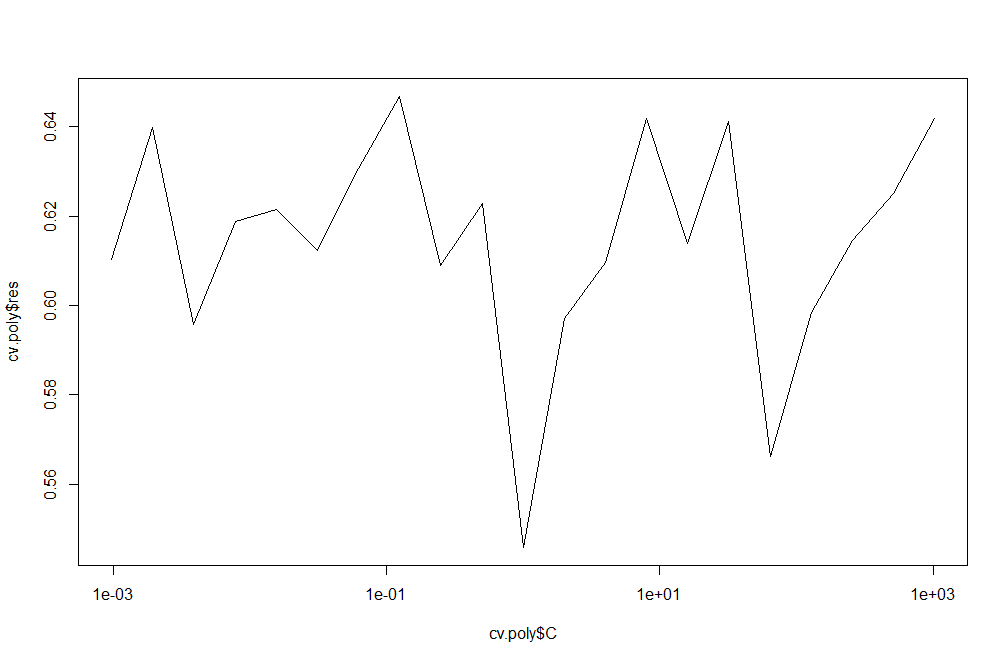
\includegraphics[scale=0.4]{auc.png}
\caption{Courbe de l'AUC pour un noyau polynomial de degré 2}
\label{fig:AUC Poly}
\end{figure}



\bibliographystyle{plain}
\bibliography{biblio} 

\end{document} 




































